% Basic setup. Most papers should leave these options alone.
%DIF LATEXDIFF DIFFERENCE FILE
%DIF DEL main_old.tex   Mon Sep  1 15:28:44 2025
%DIF ADD main.tex       Mon Sep  1 15:30:30 2025
\documentclass[fleqn,usenatbib]{mnras}

% MNRAS is set in Times font. If you don't have this installed (most LaTeX
% installations will be fine) or prefer the old Computer Modern fonts, comment
% out the following line
\usepackage{newtxtext,newtxmath}
% Depending on your LaTeX fonts installation, you might get better results with one of these:
%\usepackage{mathptmx}
%\usepackage{txfonts}

% Use vector fonts, so it zooms properly in on-screen viewing software
% Don't change these lines unless you know what you are doing
\usepackage[T1]{fontenc}

% Allow "Thomas van Noord" and "Simon de Laguarde" and alike to be sorted by "N" and "L" etc. in the bibliography.
% Write the name in the bibliography as "\VAN{Noord}{Van}{van} Noord, Thomas"
\DeclareRobustCommand{\VAN}[3]{#2}
\let\VANthebibliography\thebibliography
\def\thebibliography{\DeclareRobustCommand{\VAN}[3]{##3}\VANthebibliography}


%%%%% AUTHORS - PLACE YOUR OWN PACKAGES HERE %%%%%

% Only include extra packages if you really need them. Avoid using amssymb if newtxmath is enabled, as these packages can cause conflicts. newtxmatch covers the same math symbols while producing a consistent Times New Roman font. Common packages are:
\usepackage{graphicx}	% Including figure files
\usepackage{amsmath}	% Advanced maths commands

%%%%%%%%%%%%%%%%%%%%%%%%%%%%%%%%%%%%%%%%%%%%%%%%%%

%%%%% AUTHORS - PLACE YOUR OWN COMMANDS HERE %%%%%

% Please keep new commands to a minimum, and use \newcommand not \def to avoid
% overwriting existing commands. Example:
%\newcommand{\pcm}{\,cm$^{-2}$}	% per cm-squared

%%%%%%%%%%%%%%%%%%%%%%%%%%%%%%%%%%%%%%%%%%%%%%%%%%

%%%%%%%%%%%%%%%%%%% TITLE PAGE %%%%%%%%%%%%%%%%%%%

% Title of the paper, and the short title which is used in the headers.
% Keep the title short and informative.
\title[GPU-accelerated nested sampling for gravitational waves]{\DIFdelbegin \DIFdel{Gravitational wave }\DIFdelend \DIFaddbegin \DIFadd{Gravitational-wave }\DIFaddend inference at GPU speed: A \texttt{bilby}-like nested sampling kernel within \texttt{blackjax-ns}}

% The list of authors, and the short list which is used in the headers.
% If you need two or more lines of authors, add an extra line using \newauthor
\author[Metha Prathaban et al.]{
Metha Prathaban,$^{2,3,4}$\thanks{E-mail: myp23@cam.ac.uk (MP)}
David Yallup,$^{1,2}$
James Alvey\DIFaddbegin \DIFadd{,}\DIFaddend $^{1,2,5}$
\DIFaddbegin \DIFadd{Ming Yang,$^{1}$
Will Templeton,$^{1}$
}\DIFaddend and Will Handley$^{1,2,5}$
\\
% List of institutions
$^{1}$Institute of Astronomy, University of Cambridge, Cambridge, CB3 0HA, UK\\
$^{2}$Kavli Institute for Cosmology, University of Cambridge, Cambridge, CB3 0EZ, UK\\
$^{3}$Department of Physics, University of Cambridge, Cambridge, CB3 0HE, UK\\
$^{4}$Pembroke College, University of Cambridge, Cambridge, CB2 1RF, UK\\
$^{5}$Gonville and Caius College, University of Cambridge, Cambridge, CB2 1TA, UK\\
}

% These dates will be filled out by the publisher
\date{Accepted XXX. Received YYY; in original form ZZZ}

% Prints the current year, for the copyright statements etc. To achieve a fixed year, replace the expression with a number. 
\pubyear{\the\year{}}

% Don't change these lines
%DIF PREAMBLE EXTENSION ADDED BY LATEXDIFF
%DIF UNDERLINE PREAMBLE %DIF PREAMBLE
\RequirePackage[normalem]{ulem} %DIF PREAMBLE
\RequirePackage{color}\definecolor{RED}{rgb}{1,0,0}\definecolor{BLUE}{rgb}{0,0,1} %DIF PREAMBLE
\providecommand{\DIFadd}[1]{{\protect\color{blue}\uwave{#1}}} %DIF PREAMBLE
\providecommand{\DIFdel}[1]{{\protect\color{red}\sout{#1}}}                      %DIF PREAMBLE
%DIF SAFE PREAMBLE %DIF PREAMBLE
\providecommand{\DIFaddbegin}{} %DIF PREAMBLE
\providecommand{\DIFaddend}{} %DIF PREAMBLE
\providecommand{\DIFdelbegin}{} %DIF PREAMBLE
\providecommand{\DIFdelend}{} %DIF PREAMBLE
\providecommand{\DIFmodbegin}{} %DIF PREAMBLE
\providecommand{\DIFmodend}{} %DIF PREAMBLE
%DIF FLOATSAFE PREAMBLE %DIF PREAMBLE
\providecommand{\DIFaddFL}[1]{\DIFadd{#1}} %DIF PREAMBLE
\providecommand{\DIFdelFL}[1]{\DIFdel{#1}} %DIF PREAMBLE
\providecommand{\DIFaddbeginFL}{} %DIF PREAMBLE
\providecommand{\DIFaddendFL}{} %DIF PREAMBLE
\providecommand{\DIFdelbeginFL}{} %DIF PREAMBLE
\providecommand{\DIFdelendFL}{} %DIF PREAMBLE
\newcommand{\DIFscaledelfig}{0.5}
%DIF HIGHLIGHTGRAPHICS PREAMBLE %DIF PREAMBLE
\RequirePackage{settobox} %DIF PREAMBLE
\RequirePackage{letltxmacro} %DIF PREAMBLE
\newsavebox{\DIFdelgraphicsbox} %DIF PREAMBLE
\newlength{\DIFdelgraphicswidth} %DIF PREAMBLE
\newlength{\DIFdelgraphicsheight} %DIF PREAMBLE
% store original definition of \includegraphics %DIF PREAMBLE
\LetLtxMacro{\DIFOincludegraphics}{\includegraphics} %DIF PREAMBLE
\newcommand{\DIFaddincludegraphics}[2][]{{\color{blue}\fbox{\DIFOincludegraphics[#1]{#2}}}} %DIF PREAMBLE
\newcommand{\DIFdelincludegraphics}[2][]{% %DIF PREAMBLE
\sbox{\DIFdelgraphicsbox}{\DIFOincludegraphics[#1]{#2}}% %DIF PREAMBLE
\settoboxwidth{\DIFdelgraphicswidth}{\DIFdelgraphicsbox} %DIF PREAMBLE
\settoboxtotalheight{\DIFdelgraphicsheight}{\DIFdelgraphicsbox} %DIF PREAMBLE
\scalebox{\DIFscaledelfig}{% %DIF PREAMBLE
\parbox[b]{\DIFdelgraphicswidth}{\usebox{\DIFdelgraphicsbox}\\[-\baselineskip] \rule{\DIFdelgraphicswidth}{0em}}\llap{\resizebox{\DIFdelgraphicswidth}{\DIFdelgraphicsheight}{% %DIF PREAMBLE
\setlength{\unitlength}{\DIFdelgraphicswidth}% %DIF PREAMBLE
\begin{picture}(1,1)% %DIF PREAMBLE
\thicklines\linethickness{2pt} %DIF PREAMBLE
{\color[rgb]{1,0,0}\put(0,0){\framebox(1,1){}}}% %DIF PREAMBLE
{\color[rgb]{1,0,0}\put(0,0){\line( 1,1){1}}}% %DIF PREAMBLE
{\color[rgb]{1,0,0}\put(0,1){\line(1,-1){1}}}% %DIF PREAMBLE
\end{picture}% %DIF PREAMBLE
}\hspace*{3pt}}} %DIF PREAMBLE
} %DIF PREAMBLE
\LetLtxMacro{\DIFOaddbegin}{\DIFaddbegin} %DIF PREAMBLE
\LetLtxMacro{\DIFOaddend}{\DIFaddend} %DIF PREAMBLE
\LetLtxMacro{\DIFOdelbegin}{\DIFdelbegin} %DIF PREAMBLE
\LetLtxMacro{\DIFOdelend}{\DIFdelend} %DIF PREAMBLE
\DeclareRobustCommand{\DIFaddbegin}{\DIFOaddbegin \let\includegraphics\DIFaddincludegraphics} %DIF PREAMBLE
\DeclareRobustCommand{\DIFaddend}{\DIFOaddend \let\includegraphics\DIFOincludegraphics} %DIF PREAMBLE
\DeclareRobustCommand{\DIFdelbegin}{\DIFOdelbegin \let\includegraphics\DIFdelincludegraphics} %DIF PREAMBLE
\DeclareRobustCommand{\DIFdelend}{\DIFOaddend \let\includegraphics\DIFOincludegraphics} %DIF PREAMBLE
\LetLtxMacro{\DIFOaddbeginFL}{\DIFaddbeginFL} %DIF PREAMBLE
\LetLtxMacro{\DIFOaddendFL}{\DIFaddendFL} %DIF PREAMBLE
\LetLtxMacro{\DIFOdelbeginFL}{\DIFdelbeginFL} %DIF PREAMBLE
\LetLtxMacro{\DIFOdelendFL}{\DIFdelendFL} %DIF PREAMBLE
\DeclareRobustCommand{\DIFaddbeginFL}{\DIFOaddbeginFL \let\includegraphics\DIFaddincludegraphics} %DIF PREAMBLE
\DeclareRobustCommand{\DIFaddendFL}{\DIFOaddendFL \let\includegraphics\DIFOincludegraphics} %DIF PREAMBLE
\DeclareRobustCommand{\DIFdelbeginFL}{\DIFOdelbeginFL \let\includegraphics\DIFdelincludegraphics} %DIF PREAMBLE
\DeclareRobustCommand{\DIFdelendFL}{\DIFOaddendFL \let\includegraphics\DIFOincludegraphics} %DIF PREAMBLE
%DIF COLORLISTINGS PREAMBLE %DIF PREAMBLE
\RequirePackage{listings} %DIF PREAMBLE
\RequirePackage{color} %DIF PREAMBLE
\lstdefinelanguage{DIFcode}{ %DIF PREAMBLE
%DIF DIFCODE_UNDERLINE %DIF PREAMBLE
  moredelim=[il][\color{red}\sout]{\%DIF\ <\ }, %DIF PREAMBLE
  moredelim=[il][\color{blue}\uwave]{\%DIF\ >\ } %DIF PREAMBLE
} %DIF PREAMBLE
\lstdefinestyle{DIFverbatimstyle}{ %DIF PREAMBLE
	language=DIFcode, %DIF PREAMBLE
	basicstyle=\ttfamily, %DIF PREAMBLE
	columns=fullflexible, %DIF PREAMBLE
	keepspaces=true %DIF PREAMBLE
} %DIF PREAMBLE
\lstnewenvironment{DIFverbatim}{\lstset{style=DIFverbatimstyle}}{} %DIF PREAMBLE
\lstnewenvironment{DIFverbatim*}{\lstset{style=DIFverbatimstyle,showspaces=true}}{} %DIF PREAMBLE
%DIF END PREAMBLE EXTENSION ADDED BY LATEXDIFF

\begin{document}
\label{firstpage}
\pagerange{\pageref{firstpage}--\pageref{lastpage}}
\maketitle

% Abstract of the paper
\begin{abstract}
We present a GPU-accelerated implementation of the \DIFaddbegin \DIFadd{gravitational-wave
Bayesian inference pipeline for parameter estimation and model comparison. 
Specifically, we implement the }\DIFaddend `acceptance-walk'
sampling method, a cornerstone algorithm for gravitational-wave
inference within the \texttt{bilby} and \texttt{dynesty} framework.
By integrating this trusted kernel with the vectorized \texttt{blackjax-ns}
framework, we achieve \DIFdelbegin \DIFdel{wall-time }\DIFdelend speedups of up to two orders of
magnitude while recovering posteriors and evidences that are
statistically identical to the original CPU implementation. This faithful
re-implementation of a community-standard algorithm establishes a foundational
benchmark for gravitational-wave inference. It quantifies the
performance gains attributable solely to the architectural shift to GPUs,
\DIFdelbegin \DIFdel{thereby }\DIFdelend creating a vital reference against which future \DIFdelbegin \DIFdel{, more advanced }\DIFdelend parallel 
sampling algorithms can be rigorously assessed. 
\DIFdelbegin \DIFdel{Our results not only
demonstrate significant speedups but also serve to decouple the
effects of hardware performance from algorithmic innovation 
}\DIFdelend \DIFaddbegin \DIFadd{This allows for a clear distinction between algorithmic innovation 
and the inherent speedup from hardware, a distinction often not
explicitly drawn in other contexts such as machine learning.
Our work provides a validated tool for community use to perform
GPU-accelerated nested sampling in gravitational-wave data analyses}\DIFaddend .
\end{abstract}

% Select between one and six entries from the list of approved keywords.
% Don't make up new ones.
\begin{keywords}
keyword1 -- keyword2 -- keyword3
\end{keywords}

%%%%%%%%%%%%%%%%%%%%%%%%%%%%%%%%%%%%%%%%%%%%%%%%%%

%%%%%%%%%%%%%%%%% BODY OF PAPER %%%%%%%%%%%%%%%%%%

\section{Introduction}


The era of \DIFdelbegin \DIFdel{gravitational wave }\DIFdelend \DIFaddbegin \DIFadd{gravitational-wave }\DIFaddend (GW) astronomy, initiated by the landmark
detections \DIFdelbegin \DIFdel{of }\DIFdelend \DIFaddbegin \DIFadd{at }\DIFaddend the Laser Interferometer Gravitational-Wave Observatory (LIGO),
Virgo and now KAGRA, has revolutionized
our view of the cosmos~\citep{GW150914, GW170817,GWTC1,GWTC2, GWTC3,GWTC3_pop_analysis,GWTC2_GR,siren}. 
Extracting scientific insights from the data, from measuring the
masses and spins of binary black holes to performing precision tests of general
relativity, relies heavily on the framework of Bayesian inference~\citep{Thrane_2019}. 
This allows for the estimation of posteriors on source parameters
(parameter estimation) and the comparison of competing physical models (model selection).

The process of Bayesian inference in GW astronomy is, however, computationally
demanding. Realistic theoretical models for the GW waveform \DIFdelbegin \DIFdel{are }\DIFdelend \DIFaddbegin \DIFadd{can be }\DIFaddend complex, and the
stochastic sampling algorithms required to explore the high-dimensional parameter
space can require millions of likelihood evaluations per analysis~\citep{LIGO_guide_signalextraction}.
\DIFdelbegin \DIFdel{The }\DIFdelend \DIFaddbegin \DIFadd{There are several }\DIFaddend community-standard software tools \DIFdelbegin \DIFdel{, }\DIFdelend \DIFaddbegin \DIFadd{for performing GW inference, such as
}\texttt{\DIFadd{pycbc}}\DIFadd{~\mbox{%DIFAUXCMD
\citep{pycbc} }\hskip0pt%DIFAUXCMD
and }\texttt{\DIFadd{lal}}\DIFadd{~\mbox{%DIFAUXCMD
\citep{lal}}\hskip0pt%DIFAUXCMD
.
Here, we focus on }\DIFaddend the inference library \texttt{bilby}~\citep{bilby_paper}
paired with a custom implementation of the nested sampler \texttt{dynesty}~\citep{dynesty}, 
\DIFdelbegin \DIFdel{have }\DIFdelend \DIFaddbegin \DIFadd{which has }\DIFaddend proven to be a robust and highly effective framework, tuned for the specific needs of GW posteriors.
However, this framework is predominantly executed on central processing units
(CPUs), making individual analyses \DIFdelbegin \DIFdel{time-consuming }\DIFdelend \DIFaddbegin \DIFadd{costly }\DIFaddend and creating a
\DIFdelbegin \DIFdel{significant
}\DIFdelend computational bottleneck. This challenge is set to become acute with the
increased data volumes from future observing runs~\citep{aLIGO, aVirgo, aLVK_prospects} and the advent of
next-generation observatories, such as the Einstein Telescope~\citep{ET_science_case}, which promise
unprecedented sensitivity and detection volumes~\citep{HuAccelerationReview}.

In response to this challenge, the GW community has begun to leverage the immense
parallel processing power of graphics processing units (GPUs). Pioneering work in
this domain, such as the \texttt{jimgw} codebase~\citep{wong2023fastgravitationalwaveparameter}, has successfully
implemented GPU-accelerated Markov Chain Monte Carlo (MCMC) samplers like \texttt{flowMC}~\citep{flowMC}, 
paired with GPU implementations of waveform models provided by the
\texttt{ripple} library~\citep{ripple}. This work has demonstrated that
substantial, orders-of-magnitude speedups \DIFaddbegin \DIFadd{in runtime }\DIFaddend are
achievable for GW parameter estimation. \DIFdelbegin \DIFdel{While these MCMC-based approaches excel at rapidly generating samples
from the posterior, they do not directly compute the Bayesian evidence, which remains key for robust }\DIFdelend \DIFaddbegin \DIFadd{This success in accelerating
parameter estimation motivates the development of complementary
GPU-native algorithms to accelerate other key inference tasks, such as 
}\DIFaddend model selection.

In this paper, we introduce a GPU-accelerated nested sampling \DIFdelbegin \DIFdel{algorithm for gravitational wave }\DIFdelend \DIFaddbegin \DIFadd{(NS)
algorithm for gravitational-wave }\DIFaddend data analysis. Our method
builds upon the trusted `acceptance-walk' sampling method used in the
community-standard \texttt{bilby} and \texttt{dynesty} framework\DIFaddbegin \DIFadd{~\mbox{%DIFAUXCMD
\citep{bilby_paper}}\hskip0pt%DIFAUXCMD
}\DIFaddend .
We leverage the \texttt{blackjax-ns} sampler, a recent tool
designed for vectorized \DIFdelbegin \DIFdel{execution }\DIFdelend \DIFaddbegin \DIFadd{NS }\DIFaddend on GPUs~\citep{yallup2025nested}.
This sampler, part of the \texttt{blackjax} library, is a novel reformulation
of the core nested sampling algorithm for massive parallelization~\citep{cabezas2024blackjax}.
\DIFdelbegin %DIFDELCMD < 

%DIFDELCMD < %%%
\DIFdelend Instead of its default slice sampler, we developed a custom
kernel that implements the `acceptance-walk' method. This
ensures our sampler's logic is almost identical to the
\texttt{bilby} and \texttt{dynesty} implementation, with differences
primarily related to parallelization. This approach offers
\texttt{bilby} users a direct path to GPU-accelerated inference for the most expensive problems in GW astronomy.
They can achieve significant speedups while retaining the same
robust and trusted algorithm at the core of their analyses.

A key motivation for this work is to establish a clear performance
baseline for GPU-based nested sampling in gravitational-wave astronomy.
By adapting the community-standard \DIFdelbegin \DIFdel{`bilby`
}\DIFdelend \DIFaddbegin \texttt{\DIFadd{bilby}}
\DIFaddend `acceptance-walk' sampler for a GPU-native framework, we aim to isolate
and quantify the speedup achieved from hardware parallelization alone.
This provides a crucial reference point, enabling future work on novel
sampling algorithms to be benchmarked in a way that disentangles
algorithmic improvements from architectural performance gains.

In the following section, we summarise the core ideas
of Bayesian inference, nested sampling and GPU architectures.
We then describe the implementation of the `acceptance-walk' sampling
method in the \texttt{blackjax-ns} framework in Section~\ref{sec:methods}, and validate it against
the \texttt{bilby} and \texttt{dynesty} implementation in Section~\ref{sec:results}, discussing
our results. Finally, we present our conclusions in Section~\ref{sec:conclusions}.

\begin{figure*}
    \centering
    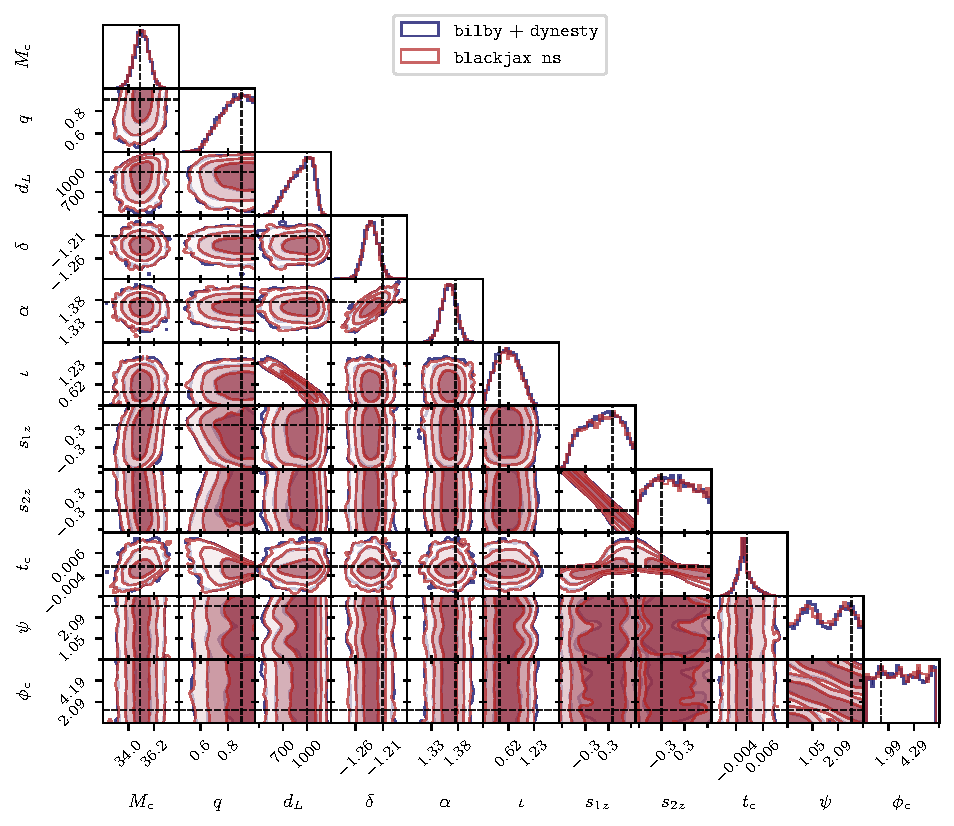
\includegraphics{figures/bilby_blackjax_comparison_4s.pdf}
    \caption{Recovered posteriors for the 4s signal. The posteriors are in \DIFdelbeginFL \DIFdelFL{agreement }\DIFdelendFL \DIFaddbeginFL \DIFaddFL{excellentagreement }\DIFaddendFL with each other, demonstrating that
    \texttt{blackjax-ns} implementation with our custom kernel is functionally equivalent to the \texttt{bilby} + \texttt{dynesty} implementation.}
    \label{fig:4s_posteriors}
\end{figure*}

\section{Background}
\label{sec:background}

\subsection{Bayesian inference in GW astronomy}
\label{sec:background_bayes}
We provide a brief overview of the core concepts of
Bayesian inference as applied to GW astronomy. For a more
comprehensive treatment, we refer the reader to~\cite{skilling, Thrane_2019, lal, bilby_paper, LIGO_guide_signalextraction}.

The analysis of GW signals is fundamentally a problem of statistical
inference, for which the Bayesian framework is the community standard.
The relationship between data, $d$, and a set of \DIFdelbegin \DIFdel{source }\DIFdelend parameters,
$\theta$, under a specific hypothesis, $H$, is given by Bayes' theorem~\citep{Bayes1763}:

\begin{equation}
    \DIFdelbegin \DIFdel{p}\DIFdelend \DIFaddbegin \DIFadd{\mathcal{P}}\DIFaddend (\theta|d, H) = \frac{\mathcal{L}(d|\theta, H) \pi(\theta|H)}{Z(d|H)}.
    \label{eq:bayes_theorem}
\end{equation}%
Here, the posterior, \DIFdelbegin \DIFdel{$p(\theta|d, H)$}\DIFdelend \DIFaddbegin \DIFadd{$\mathcal{P}(\theta|d, H)$}\DIFaddend , is the probability distribution
of the source parameters conditioned on the observed data. It is
determined by the likelihood, $\mathcal{L}(d|\theta, H)$, which is the
probability of observing the data given a specific realisation of the
model, and the prior, $\pi(\theta|H)$, which encodes initial beliefs
about the parameter distributions.

The denominator is the Bayesian evidence,
\begin{equation}
    Z(d|H) = \int \mathcal{L}(d|\theta, H) \pi(\theta|H) d\theta,
    \label{eq:evidence}
\end{equation}
defined as the likelihood integrated over the entire volume of the
prior parameter space.

There are two pillars of Bayesian inference of particular interest
in GW astronomy. The first, parameter estimation, seeks to infer 
the posterior distribution $p(\theta|d, H)$ of the source parameters of a signal or population of signals.
The second, model selection, evaluates two competing
models, $H_1$ and $H_2$, under a fully Bayesian framework by computing the ratio of
their evidences, known as the Bayes factor, $Z_1 / Z_2$. This enables
principled classification of noise versus true signals, as well as the 
comparison of different waveform models\DIFaddbegin \DIFadd{~\mbox{%DIFAUXCMD
\citep{LIGO_guide_signalextraction}}\hskip0pt%DIFAUXCMD
}\DIFaddend .

In GW astronomy, the high dimensionality of the parameter space and
the computational cost of the likelihood render the direct evaluation
of Eq.~\ref{eq:bayes_theorem} and Eq.~\ref{eq:evidence} intractable~\citep{LIGO_guide_signalextraction}.
Analysis therefore relies on stochastic sampling algorithms to
numerically approximate the posterior and evidence.

\subsection{GPU-accelerated nested sampling}

\label{sec:background_ns_and_gpus}

\subsubsection{The nested sampling algorithm}
\label{sec:background_ns}

Nested Sampling \DIFdelbegin \DIFdel{(NS) }\DIFdelend is a Monte Carlo algorithm designed to solve the
Bayesian inference problem outlined in Sec.~\ref{sec:background_bayes}.
A key strength of the NS algorithm is that it directly computes the
Bayesian evidence, $Z$, while also producing posterior samples as a
natural by-product of its execution~\DIFdelbegin \DIFdel{\mbox{%DIFAUXCMD
\citep{skilling}}\hskip0pt%DIFAUXCMD
}\DIFdelend \DIFaddbegin \DIFadd{\mbox{%DIFAUXCMD
\citep{skilling, dynamic_ns}}\hskip0pt%DIFAUXCMD
}\DIFaddend .

The algorithm starts by drawing a population of $N$ `live points'
from the prior distribution, $\pi(\theta)$. It then proceeds
iteratively. In each iteration, the live point with the lowest
likelihood value, $\mathcal{L}_{\text{min}}$, is identified. This point
is deleted from the live set and stored. It is then replaced with a
new point, drawn from the prior, but subject to the hard constraint that
its likelihood must exceed that of the deleted point,
i.e., $\mathcal{L}_{\text{new}} > \mathcal{L}_{\text{min}}$. This process
systematically traverses nested shells of increasing likelihood, with
the sequence of discarded points mapping the likelihood landscape.

The primary computational challenge within the NS algorithm is the
efficient generation of a new point from the likelihood-constrained
prior~\citep{NSNature}. The specific method used for this \DIFdelbegin \DIFdel{`inner sampling' task }\DIFdelend \DIFaddbegin \DIFadd{inner kernel }\DIFaddend is a
critical determinant of the sampler's overall efficiency and robustness\DIFaddbegin \DIFadd{~\mbox{%DIFAUXCMD
\citep{NS_methods_buchner}}\hskip0pt%DIFAUXCMD
}\DIFaddend .

\subsubsection{GPU architectures for scientific computing}
\label{sec:background_gpus}

The distinct architectures of Central Processing Units (CPUs) and
Graphics Processing Units (GPUs) offer different advantages for
computational tasks. CPUs are comprised of a few powerful cores
optimised for sequential task execution and low latency. In contrast,
GPUs feature a massively parallel architecture, containing thousands of
simpler cores designed for high-throughput computation\DIFaddbegin \DIFadd{~\mbox{%DIFAUXCMD
\citep{GPU_computing}}\hskip0pt%DIFAUXCMD
}\DIFaddend .

This architecture makes GPUs exceptionally effective for problems that can
be expressed in a Single Instruction, Multiple Data (SIMD) paradigm\DIFaddbegin \DIFadd{~\mbox{%DIFAUXCMD
\citep{CUDAGuide}}\hskip0pt%DIFAUXCMD
}\DIFaddend .
In such problems, the same operation is performed simultaneously across
a large number of data elements, leading to substantial performance
gains over serial execution on a CPU. The primary trade-off is that
algorithms must be explicitly reformulated to expose this parallelism,
and not all computational problems are amenable to vectorization.

\subsubsection{A vectorized formulation of nested sampling}
\label{sec:background_vectorized_ns}

The iterative, one-at-a-time nature of the traditional NS algorithm
is intrinsically serial, making it a poor fit for the parallel
architecture of GPUs. To overcome this limitation,\DIFdelbegin \DIFdel{Yallup et al.
}\DIFdelend \DIFaddbegin \DIFadd{~\mbox{%DIFAUXCMD
\cite{yallup2025nested}
}\hskip0pt%DIFAUXCMD
}\DIFaddend recently developed a vectorized formulation of the NS algorithm,
specifically designed for highly parallel execution within the
\texttt{blackjax} framework~\DIFdelbegin \DIFdel{\mbox{%DIFAUXCMD
\citep{yallup2025nested, cabezas2024blackjax}}\hskip0pt%DIFAUXCMD
}\DIFdelend \DIFaddbegin \DIFadd{\mbox{%DIFAUXCMD
\citep{cabezas2024blackjax}}\hskip0pt%DIFAUXCMD
}\DIFaddend .

One of the core \DIFdelbegin \DIFdel{innovations }\DIFdelend \DIFaddbegin \DIFadd{parts }\DIFaddend of this approach is the \DIFdelbegin \DIFdel{introduction }\DIFdelend \DIFaddbegin \DIFadd{idea }\DIFaddend of batch
processing. Instead of replacing a single live point in each iteration,
the algorithm removes a batch of $k$ points with the lowest likelihoods
simultaneously\DIFaddbegin \DIFadd{~\mbox{%DIFAUXCMD
\citep{parallel_ns}}\hskip0pt%DIFAUXCMD
}\DIFaddend . The critical step of replacing these points is then
parallelized. The algorithm launches $k$ independent sampling processes
on the GPU, with each process tasked with finding one new point that
satisfies the likelihood constraint, $\mathcal{L} > \mathcal{L}_{\text{min}}$,
where $\mathcal{L}_{\text{min}}$ is now the maximum likelihood of the
discarded batch.

This reformulation transforms the computationally intensive task of
sample generation from a serial challenge into a massively parallel one,
thereby leveraging the architectural strengths of the GPU. While the
original work proposed a specific inner sampling kernel\DIFaddbegin \DIFadd{, based on
Hit-and-Run Slice Sampling~\mbox{%DIFAUXCMD
\citep{Neal2003_slice}}\hskip0pt%DIFAUXCMD
, }\DIFaddend for this task,
the vectorized framework itself is general. It provides a structure
within which any suitable inner sampling \DIFdelbegin \DIFdel{method }\DIFdelend \DIFaddbegin \DIFadd{kernel }\DIFaddend can be deployed in
parallel. \DIFaddbegin \DIFadd{Here, we implement one particular method used within the }\texttt{\DIFadd{bilby}}
\DIFadd{and }\texttt{\DIFadd{dynesty}} \DIFadd{framework.
}\DIFaddend 


\section{Methods}
\label{sec:methods}

\subsection{The inner sampling kernel}
\label{sec:methods_kernel}

\begin{figure}
    \centering
    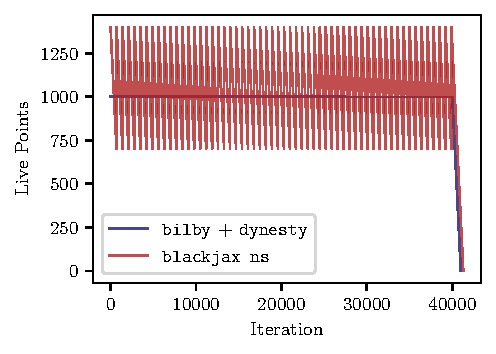
\includegraphics{figures/nlive_comparison.pdf}
    \caption{Comparison of the number of live points in the sequential CPU and batched GPU implementations.
    Although the nominal number of live points used in \texttt{blackjax-ns} is higher than in \texttt{bilby},
    the saw-tooth pattern means that the effective number of live points is the same.}
    \label{fig:nlive_comparison}
\end{figure}

Several inner sampling methods are implemented within the
\texttt{bilby} and \texttt{dynesty} framework~\citep{bilby_paper, dynesty}. In this work, we
focus on a GPU-accelerated implementation of the `acceptance-walk'
method, which is a robust and widely used choice for GW analyses.

In the standard CPU-based \texttt{dynesty} implementation, the sampler
generates a new live point by initiating a Markov Chain Monte Carlo
(MCMC) walk from the position of the deleted live point. 
The proposal mechanism for the MCMC walk is based on Differential
Evolution (DE)~\citep{DE, DE2}, which uses the distribution of existing live points to
inform jump proposals. A new candidate point is generated by adding a
scaled vector difference of two other randomly chosen live points to the
current point in the chain. Under the default \texttt{bilby} configuration, 
the scaling factor for this vector is chosen stochastically: with equal probability, 
it is either fixed at 1.0 or drawn from a \DIFaddbegin \DIFadd{scaled }\DIFaddend gamma distribution. This proposed 
point is accepted if it satisfies the likelihood constraint, $\mathcal{L} > \mathcal{L}_{\text{min}}$,
where $\mathcal{L}_{\text{min}}$ is the likelihood of the
discarded point being replaced. The \DIFaddbegin \DIFadd{sampling
process is performed in the unit hypercube space, with prior
transformations applied to evaluate the likelihood of proposed points in the physical parameter space. 
The }\DIFaddend walk length is adaptive on a per-iteration
basis; the algorithm adjusts the number of MCMC steps dynamically to
target a pre-defined number of accepted steps (e.g., 60) for each new
live point generated, up to a maximum limit.

This per-iteration adaptive strategy, however, is ill-suited for GPU
architectures. The variable walk length required for each parallel
sampler would lead to significant thread divergence, where different
cores on the GPU finish their tasks at different times, undermining the
efficiency of the SIMD execution model. To leverage GPU acceleration
effectively, the computational workload must be as uniform as possible
across all parallel processes.

Our implementation therefore preserves the core DE proposal mechanism but
modifies the walk-length adaptation to be compatible with a vectorized
framework. Within the \texttt{blackjax-ns} sampler, the number of MCMC
steps is fixed for all parallel processes within a single batch of
live point updates. The adaptive tuning is then performed at the batch
level. After a batch of $k$ new points has been generated, we compute
the mean acceptance rate across all $k$ walks. The walk length for the
subsequent batch is then adjusted based on this average rate,
using the same logic as \texttt{bilby} to target a desired number of
accepted proposals.

While this batch-adaptive approach is essential for efficient GPU
vectorization, it introduces some important differences\DIFdelbegin \DIFdel{. In the sequential CPU
algorithm, an individual MCMC walk that proves to be an outlier with a low acceptance rate
will result in a longer walk only for the iteration after it. In our parallel algorithm, if a subset of points
in a batch has a low acceptance rate, the average rate will be reduced,
causing the walk length for the entire next batch to increase. 
The converse is also true: if a subset of points in a batch has a particularly high acceptance rate, the average rate will be increased, causing the walk length for the entire next batch to decrease.
This can often lead to a very different total number of likelihood
evaluations compared to the sequential counterpart. We discuss this further in Sections~\ref{sec:sampler_config}and~\ref{sec:results}
but depending on the evidence, the likelihood evaluations can be higher or lower, and 
may need further tuning}\DIFdelend \DIFaddbegin \DIFadd{, discussed further in Section~\ref{sec:sampler_config}}\DIFaddend .
Despite this architectural modification, our kernel is designed to be functionally
analogous to the trusted \texttt{bilby} sampler\DIFdelbegin \DIFdel{, operating within the same unit hypercube space and utilizing the same DE proposal strategy
to explore the parameter space. Even in cases where
the GPU-based implementation performs more likelihood evaluations, it is significantly faster than its CPU-based counterpart}\DIFdelend \DIFaddbegin \DIFadd{. This design
represents the most direct translation of the }\texttt{\DIFadd{bilby}} \DIFadd{logic
to GPUs, making only the minimal changes required for efficient execution}\DIFaddend . 

\subsection{Sampler configuration and settings}
\label{sec:sampler_config}

The primary architectural difference between our GPU-based implementation
and the standard CPU-based `acceptance-walk' kernel is the use of
batched sampling. In our framework, a batch of $k$ new points is
run and added to the live set simultaneously. This batch size is
a user-configurable parameter, \texttt{num\_delete}, and we find that a
value of \DIFdelbegin \DIFdel{$k \approx 0.5 \times \texttt{n\_live}$ }\DIFdelend \DIFaddbegin \DIFadd{\mbox{$k \approx 0.5 \times \texttt{n\_live}$} }\DIFaddend provides a good balance
of parallel efficiency and sampling accuracy for most problems\DIFaddbegin \DIFadd{~\mbox{%DIFAUXCMD
\citep{yallup2025nested}}\hskip0pt%DIFAUXCMD
}\DIFaddend .

This batched approach has direct consequences for the adaptive tuning of
the MCMC walk length. The tuning is performed only once per \texttt{num\_delete} iterations, 
rather than at every iteration, and every point in a given batch is tuned to have the same walk length.
This design is important for preventing thread divergence and is the 
most natural way to implement this algorithm on a GPU.
However, this less frequent \DIFdelbegin \DIFdel{and more global tuning means that the standard settings for
}\DIFdelend \DIFaddbegin \DIFadd{tuning renders the standard }\DIFaddend \texttt{bilby}
\DIFdelbegin \DIFdel{parameters such as }\texttt{\DIFdel{naccept}} %DIFAUXCMD
\DIFdel{may no longer be optimal. For
instance, on high-SNR signals which require many nested sampling
iterations, the walk length can adapt to become overly long.
Conversely, on low-SNR signals that converge quickly, the sampler has
fewer opportunities to adapt, potentially resulting in a walk length
that is shorter than optimal. We discuss this behaviour and provide more
guidance on parameter settings in Sec.~\ref{sec:results}}\DIFdelend \DIFaddbegin \DIFadd{tuning parameter `delay', a smoothing factor for
the adaptation, sub-optimal. 
To achieve a comparable number of accepted steps per
iteration, we therefore adjust this parameter for the parallel
framework. The `delay' is modified to be a function of the batch size,
recovering the standard }\texttt{\DIFadd{bilby}} \DIFadd{behaviour in the sequential
limit}\DIFaddend .

Another subtle but critical consequence of \DIFdelbegin \DIFdel{this architectural shift }\DIFdelend \DIFaddbegin \DIFadd{the architectural shift to GPUs }\DIFaddend is
its effect on the evolution of the live point set. In the sequential
CPU case, the number of live points is approximately constant throughout the run. In the
batched GPU case, the number of live points follows a `saw-tooth'
pattern, decreasing from $n_{\text{live}}$ to
\DIFdelbegin \DIFdel{$n_{\text{live}} - k$ }\DIFdelend \DIFaddbegin \DIFadd{\mbox{$n_{\text{live}} - k$} }\DIFaddend over one cycle of $k$ iterations before being replenished (Fig.~\ref{fig:nlive_comparison}). This pattern
causes the effective number of live points to be lower than the nominal number,
making it appear that the sampler is able to converge faster than its sequential counterpart
when both are configured with the same number of live points.

\begin{figure}
    \centering
    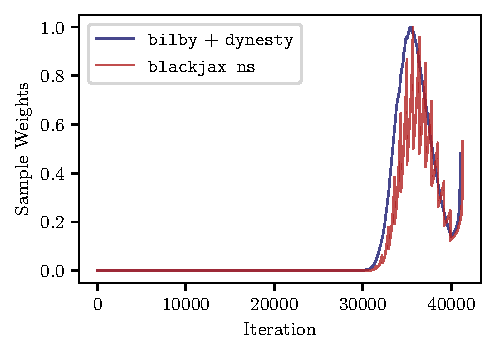
\includegraphics{figures/weights_comparison.pdf}
    \caption{Comparison of the sample weights for each dead point for the sequential CPU and batched GPU implementations.
    The weights are calculated using the prior volumes enclosed between successive dead points \DIFaddbeginFL \DIFaddFL{and the likelihoods}\DIFaddendFL . 
    The shapes are similar, and both implementations enter the bulk of the posterior distribution at similar iterations,
    indiciating that setting the number of live points in \texttt{blackjax-ns} to 1.4 times the number of live points in \texttt{bilby} 
    does indeed result in a like-for-like comparison. The same saw-tooth pattern can be 
    seen in the weights for the \texttt{blackjax-ns} implementation.}
    \label{fig:weights_comparison}
\end{figure}
%\vspace{-0.25cm}

To conduct a fair and direct comparison between the two frameworks, this
discrepancy must be accounted for. We therefore adjust the number of
live points in the GPU sampler, $n_{\text{GPU}}$, such that the
expected prior volume compression matches that of the CPU sampler. 
Under these settings, both implementations will converge in
approximately the same number of nested sampling iterations (see Figure~\ref{fig:weights_comparison}). 
The following derivation outlines this adjustment.

\subsubsection{Setting $n_{\text{GPU}}$}
\label{sec:setting_n_gpu}

The expected log prior volume fraction, $\log X$, remaining after $k$ iterations
of a nested sampling run is given by~\DIFdelbegin \DIFdel{\mbox{%DIFAUXCMD
\citep{skilling}
}\hskip0pt%DIFAUXCMD
}\DIFdelend \DIFaddbegin \DIFadd{\mbox{%DIFAUXCMD
\citep{skilling, dynamic_ns, aeons}
}\hskip0pt%DIFAUXCMD
}\DIFaddend \begin{equation}
    E[\log X_k] = \sum_{i=1}^{k} \frac{1}{n_i},
\end{equation}
where $n_i$ is the number of live points at iteration $i$. In the
CPU-based implementation, \DIFdelbegin \DIFdel{$n_i \approx n_{\text{CPU}}$ }\DIFdelend \DIFaddbegin \DIFadd{$n_i = n_{\text{CPU}}$ }\DIFaddend is constant.
After $k$ iterations, the expected log volume fraction is therefore
\begin{equation}
    \log X_{\text{CPU}} = \frac{k}{n_{\text{CPU}}}.
\end{equation}
\DIFdelbegin %DIFDELCMD < 

%DIFDELCMD < %%%
\DIFdelend In our GPU implementation, the number of live points decreases over one
batch cycle of $k = \texttt{num\_delete}$ iterations. The total log
volume shrinkage over one such cycle is the sum over the decreasing
number of live points:
\begin{equation}
    \log X_{\text{GPU}} = \sum_{i=0}^{k-1} \frac{1}{n_{\text{GPU}}-i} \approx \ln\left(\frac{n_{\text{GPU}}}{n_{\text{GPU}}-k}\right).
\end{equation}
To ensure a fair comparison, we equate the expected shrinkage of both
methods over one cycle of $k$ iterations:
\begin{equation}
    \frac{k}{n_{\text{CPU}}} \approx \ln\left(\frac{n_{\text{GPU}}}{n_{\text{GPU}}-k}\right).
\end{equation}
Using our recommended setting of $k = 0.5 \times n_{\text{GPU}}$, this
simplifies to $0.5 \times n_{\text{GPU}} / n_{\text{CPU}} \approx \ln(2)$.
We can therefore derive the required number of live points for the GPU
sampler to be
\begin{equation}
    n_{\text{GPU}} \approx 2 \ln(2) \times n_{\text{CPU}} \approx 1.4 \times n_{\text{CPU}}.
\end{equation}
In all comparative analyses presented in this paper, we configure the
number of live points according to this relation to ensure an equal 
\textit{effective} number of live points and
like-for-like timing comparisons.

\subsection{Likelihood}

To assess the performance of our framework, we employ a standard
frequency-domain likelihood. The total
speedup in our analysis is achieved by accelerating the two primary
computational components of the inference process: the sampler and the
likelihood evaluation. The former is parallelized at the batch level as
described in Sec.~\ref{sec:methods_kernel}, while the latter is
accelerated using a GPU-native waveform generator.

For this purpose, we generate gravitational waveforms using the
\texttt{ripple} library, which provides GPU-based implementations of
common models~\DIFdelbegin \DIFdel{\mbox{%DIFAUXCMD
\citep{ripple}}\hskip0pt%DIFAUXCMD
}\DIFdelend \DIFaddbegin \DIFadd{\mbox{%DIFAUXCMD
\citep{ripple, wong2023fastgravitationalwaveparameter, Wouters_BNS}}\hskip0pt%DIFAUXCMD
}\DIFaddend . 
This allows the waveform to be calculated
in parallel across the frequency domain \DIFaddbegin \DIFadd{and 
across multiple sets of parameters}\DIFaddend , enabling massive efficiency gains by 
ensuring that this calculation does not become a serial bottleneck.
To isolate the speedup from this combined GPU-based framework,
we deliberately avoid other established acceleration methods like 
heterodyning~\citep{TL_relativebinning, relativebinning2, relativebinning3, relativebinning4}, 
though these are available in the \texttt{\DIFdelbegin \DIFdel{ripple}\DIFdelend \DIFaddbegin \DIFadd{jimgw}\DIFaddend } library too\DIFaddbegin \DIFadd{~\mbox{%DIFAUXCMD
\citep{wong2023fastgravitationalwaveparameter}}\hskip0pt%DIFAUXCMD
}\DIFaddend .

For the analyses in this paper, we restrict our consideration to binary
black hole systems with aligned spins, for which we use the
\texttt{IMRPhenomD} waveform approximant~\citep{Khan:2015jqa}.
Further details on the specific likelihood configuration for each
analysis, including noise curves and data segments, are provided in Section~\ref{sec:results}.

\subsection{Priors}

For this initial study, we adopt a set of standard, separable priors on
the source parameters, which are summarized in Table~\ref{tab:priors}.
The specific ranges for these priors are dependent on the duration of the signal, and are
also given in Section~\ref{sec:results}.

As is the default within the \texttt{bilby} framework, we sample directly in chirp mass, $\mathcal{M}$, and
mass ratio, $q$. We use priors that are uniform in these parameters directly, instead of uniform in the component masses. 
The aligned spin components, $\chi_1$ and $\chi_2$, are also taken to be uniform over
their allowed range.The coalescence time, $t_c$, is assumed to be uniform
within a narrow window around the signal trigger time.

For the luminosity distance, $d_L$, we adopt a power-law prior of the
form $p(d_L) \propto d_L^2$. This prior corresponds to a distribution of
sources that is uniform in a Euclidean universe. While this is a
simplification that is less accurate at higher redshifts~\citep{bilby_validation}, it is a
standard choice for many analyses and serves as a robust baseline for
this work.

These priors were chosen to facilitate a direct, like-for-like
comparison against the CPU-based \texttt{bilby} and \texttt{dynesty}
framework, and in all such comparisons identical priors were used. The
implementation of more astrophysically motivated, complex prior
distributions for mass, spin, and luminosity distance is left to
future work \DIFaddbegin \DIFadd{and is independent of the algorithmic performance}\DIFaddend .

\DIFdelbegin %DIFDELCMD < \begin{table}[h!]
%DIFDELCMD < %%%
\DIFdelendFL \DIFaddbeginFL \begin{table}
\DIFaddendFL \setlength{\tabcolsep}{3pt} % Reduce space between columns (default is 6pt)
\centering
\caption{Prior distributions for the parameters of the binary black hole
system. The specific ranges for the masses and spins
 are dependent on the \DIFdelbeginFL \DIFdelFL{injection }\DIFdelendFL \DIFaddbeginFL \DIFaddFL{signal }\DIFaddendFL and are specified in Section~\ref{sec:results}.}
\label{tab:priors}
\begin{tabular}{l l l c c}
\hline
\hline
\textbf{Parameter} & \textbf{Description} & \textbf{Prior Distribution} & \textbf{Range}\\
\hline
$M_c$ & Chirp Mass & Uniform & - \\
$q$ & Mass Ratio & Uniform & - \\
$\chi_1, \chi_2$ & Aligned spin components & Uniform & - \\
$d_L$ & Luminosity Distance & Power Law (2) & [100, 5000] Mpc \\
$\theta_{\textrm{JN}}$ & Inclination Angle & Sine & [0, $\pi$] rad \\
$\psi$ & Polarization Angle & Uniform & [0, $\pi$] rad \\
$\phi_c$ & Coalescence Phase & Uniform & [0, 2$\pi$] rad \\
$t_c$ & Coalescence Time & Uniform & [-0.1, 0.1] s\\
$\alpha$ & Right Ascension & Uniform & [0, 2$\pi$] rad \\
$\delta$ & Declination & Cosine & [-$\pi$/2, $\pi$/2] rad \\
\hline
\hline
\end{tabular}
\end{table}


\section{Results and discussion}
\label{sec:results}

We now validate the performance of our framework through a series of
analyses. In all of the below results, the \texttt{bilby} analyses
were executed on a 16-core CPU instance using Icelake nodes, while the \texttt{blackjax-ns}
analyses were performed on a single NVIDIA L4 GPU, unless otherwise specified.

\subsection{Simulated signals}

\subsubsection{4-second simulated signal}
\label{sec:4s_simulated_signal}

We begin by analysing a 4-second simulated signal from a binary black
hole (BBH) merger. The injection parameters for this signal are
detailed in Table~\ref{tab:injection_params}. To ensure a direct,
like-for-like comparison, the signal was injected into simulated
detector noise using the \texttt{bilby} library, and 
then loaded into both sets of analyses. The analysis
uses a three-detector network, with the design
sensitivity for the fourth LIGO-Virgo-KAGRA observing run (O4).
The frequency range of data analysed is from 20 Hz to 1024 Hz, 
and the network matched filtered SNR is 39.6. 

Both the CPU and GPU-based analyses were configured with 1000 \DIFdelbegin \textit{\DIFdel{effective}} %DIFAUXCMD
\DIFdelend \DIFaddbegin \DIFadd{effective }\DIFaddend live
points. As detailed in Sec.~\ref{sec:setting_n_gpu}, this corresponded to
setting the number of live points in \texttt{blackjax-ns} to 1400, with \DIFdelbegin \texttt{\DIFdel{num\_delete}} %DIFAUXCMD
\DIFdel{= 700.
}\DIFdelend \DIFaddbegin \DIFadd{\mbox{\texttt{num\_delete} = 700}.
}\DIFaddend The termination condition in both cases was set to dlogZ < 0.1, the default in \texttt{bilby},
and we used the settings \DIFdelbegin \texttt{\DIFdel{naccept}} %DIFAUXCMD
\DIFdel{= 60, }\texttt{\DIFdel{maxmcmc}} %DIFAUXCMD
\DIFdel{= 5000 and }\texttt{\DIFdel{use\_ratio = True}}%DIFAUXCMD
\DIFdelend \DIFaddbegin \DIFadd{\mbox{\texttt{naccept} = 60}, \mbox{\texttt{maxmcmc} = 5000} and \mbox{\texttt{use\_ratio = True}}}\DIFaddend . 
In both cases, periodic boundary conditions were used for the right ascension, 
polarization angle, and coalescence phase parameters. The prior ranges
for the chirp mass and mass ratio were set to $[25.0, 50.0]~M_{\odot}$
and $[0.25, 1.0]$, respectively, with \DIFdelbegin \DIFdel{uniform }\DIFdelend priors on the aligned
spin components over the range $[-1, 1]$. 

The recovered posterior distributions, shown in
Figure~\ref{fig:4s_posteriors}, demonstrate excellent statistical
agreement between the two frameworks. This result validates that our
custom `acceptance-walk' kernel within the vectorized \texttt{blackjax-ns}
framework is functionally equivalent to the trusted sequential
implementation in \texttt{bilby}. The computed log-evidence values are
also in strong agreement, as shown in Figure~\ref{fig:4s_logZ_comparison},
confirming that our implementation provides a robust unified framework for both
parameter estimation and model selection. 

The CPU-based \texttt{bilby} run completed in 2.99 hours on 16 cores, for a total of
47.8 CPU-hours. In contrast, the GPU-based \texttt{blackjax-ns} run
completed in \DIFdelbegin \DIFdel{0.8 }\DIFdelend \DIFaddbegin \DIFadd{1.25 }\DIFaddend hours. This corresponds to a \DIFdelbegin \DIFdel{wall-time }\DIFdelend \DIFaddbegin \DIFadd{sampling time }\DIFaddend speedup factor
of $\times$\DIFdelbegin \DIFdel{60. In this case, the batch-adaptive nature of the GPU
sampler led to a
slightly higher number of likelihood evaluations
(70.6 million) compared to the sequential CPU sampler (}\DIFdelend \DIFaddbegin \DIFadd{38. The }\texttt{\DIFadd{bilby}} \DIFadd{and }\texttt{\DIFadd{blackjax-ns}} \DIFadd{runs performed
}\DIFaddend 62.9 \DIFdelbegin \DIFdel{million)}\DIFdelend \DIFaddbegin \DIFadd{million and 62.5 million likelihood evaluations and had a
mean number of accepted steps per iteration of 28.5 and 30.7, respectively}\DIFaddend .

Beyond \DIFdelbegin \DIFdel{wall-time}\DIFdelend \DIFaddbegin \DIFadd{sampling time}\DIFaddend , we also consider the relative financial cost. Based
on commercial on-demand rates from Google Cloud, the rental cost for the 16-core
CPU instance and the L4 GPU instance were approximately equivalent at
the time of this work. This equivalence in hourly cost implies a direct
cost-saving factor of approximately $\times$\DIFdelbegin \DIFdel{3.7 }\DIFdelend \DIFaddbegin \DIFadd{2.4 }\DIFaddend for the GPU-based analysis.

In the interest of benchmarking, we also performed the analysis on 
an A100 NVIDIA GPU configured with the same run settings as the L4 GPU.
The A100 is a more powerful GPU, resulting in a lower runtime. Interestingly,
however, when comparing the relative commercial hourly rates of the two GPUs,
the L4 GPU analysis was actually cheaper. \DIFaddbegin \DIFadd{The A100 analysis had a 
worse cost to the CPU implementation. }\DIFaddend We summarise these results in 
Table~\ref{tab:4s_time_comparison}.

\begin{table}
    \centering
    \caption{Injection parameters for the 4s signal.}
    \label{tab:injection_params}
    \begin{tabular}{l l l c c}
    \hline
    \hline
    \textbf{Parameter} & \textbf{Value} \\
    \hline
    $\mathcal{M}$ & 35.0 M$_{\odot}$ \\
    $q$ & 0.90 \\
    $\chi_1$ & 0.40 \\
    $\chi_2$ & -0.30 \\
    $d_L$ & 1000 Mpc \\
    $\theta_{\textrm{JN}}$ & 0.40 rad \\
    $\psi$ & 2.66 rad \\
    $\phi$ & 1.30 rad \\
    $t_c$ & 0.0 s\\
    $\alpha$ & 1.38 rad \\
    $\delta$ & -1.21 rad \\
    \hline
    \hline
    \end{tabular}
    \end{table}

\begin{figure}
    \centering
    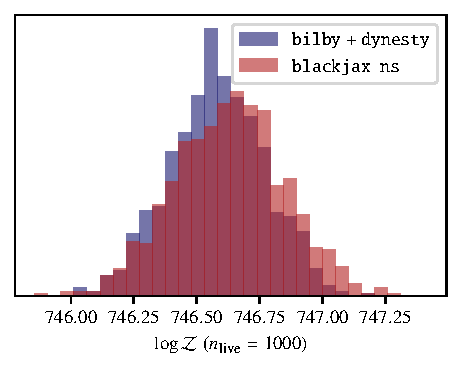
\includegraphics{figures/4s_logZ_comparison.pdf}
    \caption{Comparison of the log evidence for the 4s signal. The results are in excellent agreement, demonstrating the
    robustness of the \texttt{blackjax-ns} implementation in recovering the same posteriors and evidence as the \texttt{bilby} implementation.
    This unifies parameter estimation and evidence evaluation into a single GPU-accelerated framework.}
    \label{fig:4s_logZ_comparison}
\end{figure}

\begin{table}
    \setlength{\tabcolsep}{3pt}
    \centering
    \caption{Comparison of the \DIFdelbeginFL \DIFdelFL{wall-times }\DIFdelendFL \DIFaddbeginFL \DIFaddFL{sampling times }\DIFaddendFL and cost savings for the 4s signal.}
    \label{tab:4s_time_comparison}
    \begin{tabular}{l l l c c}
    \hline
    \hline
    \textbf{Implementation + Hardware} & \textbf{\DIFdelbeginFL \DIFdelFL{Wall-time }\DIFdelendFL \DIFaddbeginFL \DIFaddFL{Time }\DIFaddendFL (h)} & \textbf{Speedup} & \textbf{Cost Saving} \\
    \hline
    \texttt{bilby} (16 Icelake CPU cores) & 47.8 & - & - \\
    \texttt{blackjax-ns} (NVIDIA L4) & \DIFdelbeginFL \DIFdelFL{0.8 }\DIFdelendFL \DIFaddbeginFL \DIFaddFL{1.25 }\DIFaddendFL & \DIFdelbeginFL \DIFdelFL{60}\DIFdelendFL \DIFaddbeginFL \DIFaddFL{38}\DIFaddendFL $\times$ & \DIFdelbeginFL \DIFdelFL{3.7}\DIFdelendFL \DIFaddbeginFL \DIFaddFL{2.4}\DIFaddendFL $\times$ \\
    \texttt{blackjax-ns} (NVIDIA A100) & \DIFdelbeginFL \DIFdelFL{0.6 }\DIFdelendFL \DIFaddbeginFL \DIFaddFL{0.93 }\DIFaddendFL & \DIFdelbeginFL \DIFdelFL{80}\DIFdelendFL \DIFaddbeginFL \DIFaddFL{51}\DIFaddendFL $\times$ & \DIFdelbeginFL \DIFdelFL{5}\DIFdelendFL \DIFaddbeginFL \DIFaddFL{0.6}\DIFaddendFL $\times$ \\
    \hline
    \hline
    \end{tabular}
    \end{table}


\subsection{Injection Study}
\label{sec:injection_study}

To systematically assess the performance and robustness of our framework
across a diverse parameter space, we performed an injection study
comparing our GPU-based \texttt{blackjax-ns} sampler against the
CPU-based \texttt{bilby}+\texttt{dynesty} implementation. A population
of 100 simulated BBH signals was generated using \texttt{bilby} and
injected into noise representative of the O4 detector network
sensitivity. The network signal-to-noise ratios (SNR) for this
injection set span a range from 1.84 to 17.87 (Figure~\ref{fig:snr_dist}).
As above, we use a three-detector network for the analysis.

\begin{figure}
    \centering
    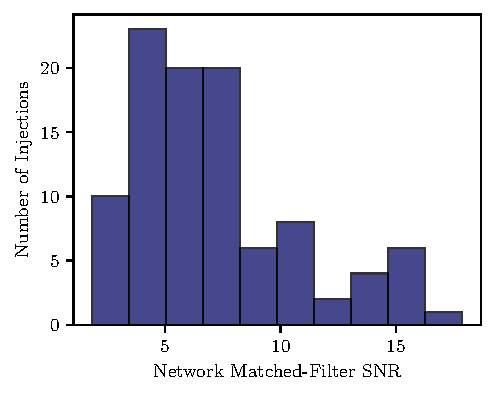
\includegraphics{figures/injection_snr_hist.pdf}
    \caption{Distribution of the network signal-to-noise ratios (SNR) for the injected signals.}
    \label{fig:snr_dist}
\end{figure}


For this study, the prior ranges were set to $[20.0, 50.0]~M_{\odot}$
for the chirp mass and $[0.5, 1.0]$ for the mass ratio. The aligned
spin components were bounded by uniform priors over the range
$[-0.8, 0.8]$. All other prior distributions are as defined in
Table~\ref{tab:priors}.

All analyses in this study were performed using 1000 live points for \texttt{bilby} and
1400 live points for \texttt{blackjax-ns}. Given that quite a few signals in the set have a low SNR, and therefore a
low Bayes factor comparing the signal hypothesis to the noise-only
hypothesis, a more robust termination condition was required to
ensure accurate evidence computation as well as posterior estimation.
We therefore set the termination criterion based on the fractional
remaining evidence, such that the analysis stops when the estimated
evidence in the live points is less than 0.1\% of the accumulated
evidence. \DIFdelbegin %DIFDELCMD < 

%DIFDELCMD < %%%
\DIFdel{In the first instance, both }\DIFdelend \DIFaddbegin \DIFadd{Both }\DIFaddend samplers were configured with
\DIFdelbegin \texttt{\DIFdel{naccept}} %DIFAUXCMD
\DIFdel{= 60 and }\texttt{\DIFdel{maxmcmc}} %DIFAUXCMD
\DIFdel{= 5000}\DIFdelend \DIFaddbegin \DIFadd{\mbox{\texttt{naccept} = 60} and \mbox{\texttt{maxmcmc} = 5000}}\DIFaddend , and the \texttt{blackjax-ns}
sampler used a batch size of \DIFdelbegin \texttt{\DIFdel{num\_delete}} %DIFAUXCMD
\DIFdel{= 700. The posterior
distributions were in good agreement with each other and the 
percentile-percentile (PP) plot was unbiased. However, due to the low SNR and 
the algorithmic differences arising from parallelisation,
we found that the mean accepted steps per iteration was lower in }\texttt{\DIFdel{blackjax-ns}}
%DIFAUXCMD
\DIFdel{compared to }\texttt{\DIFdel{bilby}}%DIFAUXCMD
\DIFdel{, leading to an unfair comparison in the runtimes. We therefore applied more aggressive tuning to the 
}\texttt{\DIFdel{blackjax-ns}} %DIFAUXCMD
\DIFdel{chain lengths to compensate for the limited number of opportunities
to perform the tuning, and re-ran the analysis. In practice, this was achieved by setting }\texttt{\DIFdel{naccept}} %DIFAUXCMD
\DIFdel{= 120
for the }\texttt{\DIFdel{blackjax-ns}} %DIFAUXCMD
\DIFdel{runs. This resulted in a similar number of likelihood evaluations
and accepted steps per iteration to }\texttt{\DIFdel{bilby}} %DIFAUXCMD
\DIFdel{(see Figure~\ref{fig:chain_length_comparison}), enabling a fairer and more direct comparison
of the two implementations. 
For low SNR signals, we therefore recommend setting }\texttt{\DIFdel{naccept}} %DIFAUXCMD
\DIFdel{to a higher value to ensure
similar run properties to }\texttt{\DIFdel{bilby}}%DIFAUXCMD
\DIFdelend \DIFaddbegin \DIFadd{\mbox{\texttt{num\_delete} = 700}}\DIFaddend . 



\begin{figure}
    \centering
    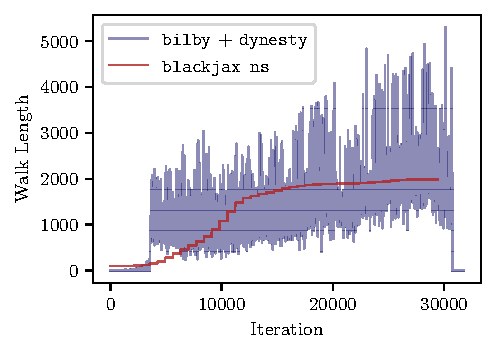
\includegraphics{figures/chain_length_comparison.pdf}
    \caption{Comparison of the \DIFdelbeginFL \DIFdelFL{chain lengths }\DIFdelendFL \DIFaddbeginFL \DIFaddFL{accepted number of steps per iteration }\DIFaddendFL for the sequential CPU and batched GPU implementations.
    \DIFaddbeginFL \DIFaddFL{We adapt our `delay' parameter from the tuning formula such that we obtain similar accepted steps for the 
    two implementations. }\DIFaddendFL The \texttt{blackjax-ns} implementation can only perform \DIFdelbeginFL \DIFdelFL{batch }\DIFdelendFL tuning \DIFaddbeginFL \DIFaddFL{every \mbox{\texttt{num\_delete}} iterations}\DIFaddendFL ,
    \DIFdelbeginFL \DIFdelFL{a fundamental algorithmic difference 
   between the CPU-based and GPU-based implementations of the `acceptance-walk' kernel. This leads to a staircase
   pattern in the chain lengths, which can be seen in }\DIFdelendFL \DIFaddbeginFL \DIFaddFL{so we tune }\DIFaddendFL the \DIFdelbeginFL \DIFdelFL{plot. However, setting }\texttt{\DIFdelFL{naccept}} %DIFAUXCMD
\DIFdelFL{= 120 in }\texttt{\DIFdelFL{blackjax-ns}}
   %DIFAUXCMD
\DIFdelFL{and }\texttt{\DIFdelFL{naccept}} %DIFAUXCMD
\DIFdelFL{= 60 in }\texttt{\DIFdelFL{bilby}} %DIFAUXCMD
\DIFdelFL{results in similar average }\DIFdelendFL chain \DIFdelbeginFL \DIFdelFL{lengths for the injection study}\DIFdelendFL \DIFaddbeginFL \DIFaddFL{length more aggressively}\DIFaddendFL .}
    \label{fig:chain_length_comparison}
\end{figure}

The resulting PP plot for our \texttt{blackjax-ns} sampler
with the `acceptance-walk' kernel is shown in Figure~\ref{fig:pp_coverage}.
This plot evaluates the self-consistency of the posteriors by checking
the distribution of true injected parameter values within their
recovered credible intervals. The results demonstrate that the credible
intervals are well-calibrated, with the cumulative distributions for all
parameters lying within the expected statistical variance of the
line of perfect calibration. This confirms the robustness of our implementation. The full
set of posterior and evidence results for all 100 injections is made
publicly available in the data repository accompanying this paper\DIFdelbegin \DIFdel{.
\textcolor{red}{TODO: add link/ref}
}\DIFdelend \DIFaddbegin \DIFadd{~\mbox{%DIFAUXCMD
\citep{Prathaban_2025_zenodo}}\hskip0pt%DIFAUXCMD
.
}\DIFaddend 

\begin{figure}
    \centering
    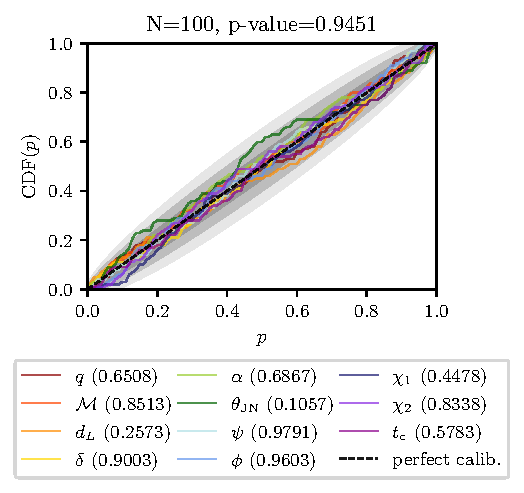
\includegraphics[width=\columnwidth]{figures/pp_coverage_blackjax.pdf}
    \caption{Percentile-percentile (PP) coverage plot for the
    100-injection study, obtained with the \texttt{blackjax-ns}
    sampler. The cumulative fraction of events where the true
    injected parameter falls below a given credible level is plotted
    against that credible level. The proximity of all parameter curves
    to the diagonal indicates that the posterior credible intervals
    are statistically well-calibrated. A corresponding plot for the
    \texttt{bilby+dynesty} analysis, which should be identical,
    is provided in the Appendix for reference.}
    \label{fig:pp_coverage}
\end{figure}

\begin{figure}
    \centering
    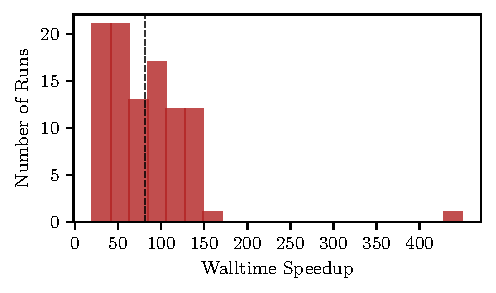
\includegraphics{figures/walltime_speedup.pdf}
    \caption{The wall-time speedups for all 100 events in the injection study.}
    \label{fig:speedup_comparison}
\end{figure}

\begin{figure}
    \centering
    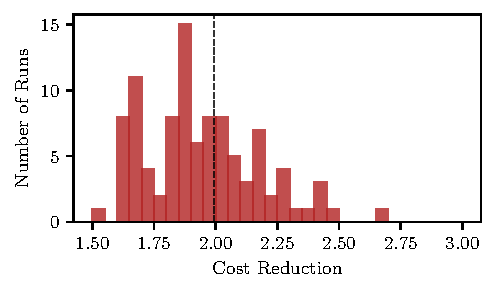
\includegraphics{figures/cost_reduction.pdf}
    \caption{The cost reductions for all 100 events in the injection study.}
    \label{fig:cost_reduction}
\end{figure}

The average chain length for the \texttt{blackjax-ns}
sampler was 1376, consistent with the average of 1337 for the
\texttt{bilby+dynesty} sampler. A more detailed breakdown of all run
statistics is provided in Appendix~\ref{app:injection_study_stats}.
In terms of \DIFdelbegin \DIFdel{wall-time}\DIFdelend \DIFaddbegin \DIFadd{runtime}\DIFaddend , the \texttt{blackjax-ns} sampler completed the analyses
in an average of 0.4 hours per injection, with individual run
times ranging from 9 to 56 minutes.
In contrast, the CPU-based runs
required an average of 26.4 total CPU-hours, with some runs taking as long as 
100 hours. 
Figure~\ref{fig:speedup_comparison} shows the distribution of the
resulting \DIFdelbegin \DIFdel{wall-time }\DIFdelend \DIFaddbegin \DIFadd{runtime }\DIFaddend speedup factors, which have a mean value of
$\times$81.2. As in 
section~\ref{sec:4s_simulated_signal}, we also translate this performance 
gain into a cost reduction using commercial cloud computing rates.
As shown in Figure~\ref{fig:cost_reduction}, the speedup
corresponds to an average cost-reduction factor of $\times$5.1 for the
GPU-based analysis compared to its CPU-based counterpart.

\subsection{Disentangling Sources of GPU Acceleration}
\label{sec:disentangling_acceleration}

The overall performance gain of our framework arises from two distinct
forms of parallelisation: the parallel evaluation of a single
likelihood across its frequency bins (intra-likelihood), and the
parallel sampling process itself, where multiple MCMC chains are run
simultaneously (inter-sample). In this section, we attempt to disentangle
these two contributions.

We configured our \texttt{blackjax-ns} sampler to run in a sequential
mode. This was achieved by setting the batch size to one
(\texttt{num\_delete} = 1) and the number of live points to 1000,
identical to the CPU analysis. With a batch size of one, the
`saw-tooth' pattern in the live point population described in
Sec.~\ref{sec:sampler_config} is eliminated, making the effective
number of live points equal to the nominal value. This removes the need
for the corrective scaling of $n_{\text{live}}$ applied in our main
parallel analyses\DIFaddbegin \DIFadd{, and we can also use the same }\texttt{\DIFadd{naccept}}
\DIFadd{value as for the }\texttt{\DIFadd{bilby}} \DIFadd{runs}\DIFaddend . In this configuration, the algorithm proceeds
analogously to the \texttt{bilby} implementation, and the only source of
acceleration relative to the CPU is the GPU's ability to parallelise the
likelihood calculation over the frequency domain.

For this test, we used the first signal from our injection study (network
SNR of 8.82). The baseline CPU-based \texttt{bilby} analysis required
30.4 total CPU-hours to complete. The sequential-GPU analysis, which
benefits only from intra-likelihood parallelisation, completed in
10.44 hours. This represents a speedup of $\times$2.9. Finally, the
fully parallel run, using its correctly scaled live point count of 1400\DIFdelbegin \DIFdel{and }\DIFdelend \DIFaddbegin \DIFadd{,
}\DIFaddend a batch size of \texttt{num\_delete} = 700 \DIFaddbegin \DIFadd{and }{\texttt{\DIFadd{naccept}} \DIFadd{= 120}}\DIFaddend , completed in \DIFdelbegin \DIFdel{0.45 }\DIFdelend \DIFaddbegin \DIFadd{1.29 }\DIFaddend hours.
This corresponds to a further speedup of $\times$\DIFdelbegin \DIFdel{23.2 }\DIFdelend \DIFaddbegin \DIFadd{8.1 }\DIFaddend over the
sequential-GPU run.

This result demonstrates that while a GPU-native likelihood provides
a significant performance benefit, the \DIFaddbegin \DIFadd{more }\DIFaddend dominant contribution to the
overall speedup (a total of $\times$\DIFdelbegin \DIFdel{67.6 }\DIFdelend \DIFaddbegin \DIFadd{23.6 }\DIFaddend in this case) originates from the
massively parallel, batched sampling architecture. This result
underscores the importance of the algorithmic reformulation 
of nested sampling pioneered in~\cite{yallup2025nested}.


\subsection{8-second simulated signal}
\label{sec:8s_simulated_signal}

To investigate the scalability of our framework with a more
computationally demanding likelihood, we now analyse a simulated
8-second BBH signal. The injection parameters are detailed in
Table~\ref{tab:8s_injection_params}. For this analysis, the data are
evaluated between 20 Hz and 2048 Hz, quadrupling the number of
frequency bins compared to the 4-second signal analysis. As above, the signal was
injected into noise from a three-detector network with O4 sensitivity,
resulting in a network SNR of 11.25.

The prior ranges for the chirp mass and mass ratio were set to
$[10.0, 25.0]~M_{\odot}$ and $[0.25, 1.0]$, respectively. The aligned
spin components were bounded by uniform priors over the range
$[-0.8, 0.8]$, with all other prior distributions as defined in
Table~\ref{tab:priors}. The sampler configurations were identical to
those used in the injection study (Sec.~\ref{sec:injection_study}), with
$n_{\text{live}}=1400$ for \texttt{blackjax-ns} and
$n_{\text{live}}=1000$ for \texttt{bilby}, and an \texttt{naccept}
target of 120 and 60, respectively. In this case, we revert to the 
default termination condition described in Section~\ref{sec:4s_simulated_signal}.

\begin{table}
    \centering
    \caption{Injection parameters for the 8s signal.}
    \label{tab:8s_injection_params}
    \begin{tabular}{l l l c c}
    \hline
    \hline
    \textbf{Parameter} & \textbf{Value} \\
    \hline
    $\mathcal{M}$ & 10.0 M$_{\odot}$ \\
    $q$ & 0.70 \\
    $\chi_1$ & -0.34 \\
    $\chi_2$ & 0.01 \\
    $d_L$ & 500 Mpc \\
    $\theta_{\textrm{JN}}$ & 1.30 rad \\
    $\psi$ & 1.83 rad \\
    $\phi$ & 5.21 rad \\
    $t_c$ & 0.0 s\\
    $\alpha$ & 1.07 rad \\
    $\delta$ & -1.01 rad \\
    \hline
    \hline
    \end{tabular}
    \end{table}

\begin{figure*}
    \centering
    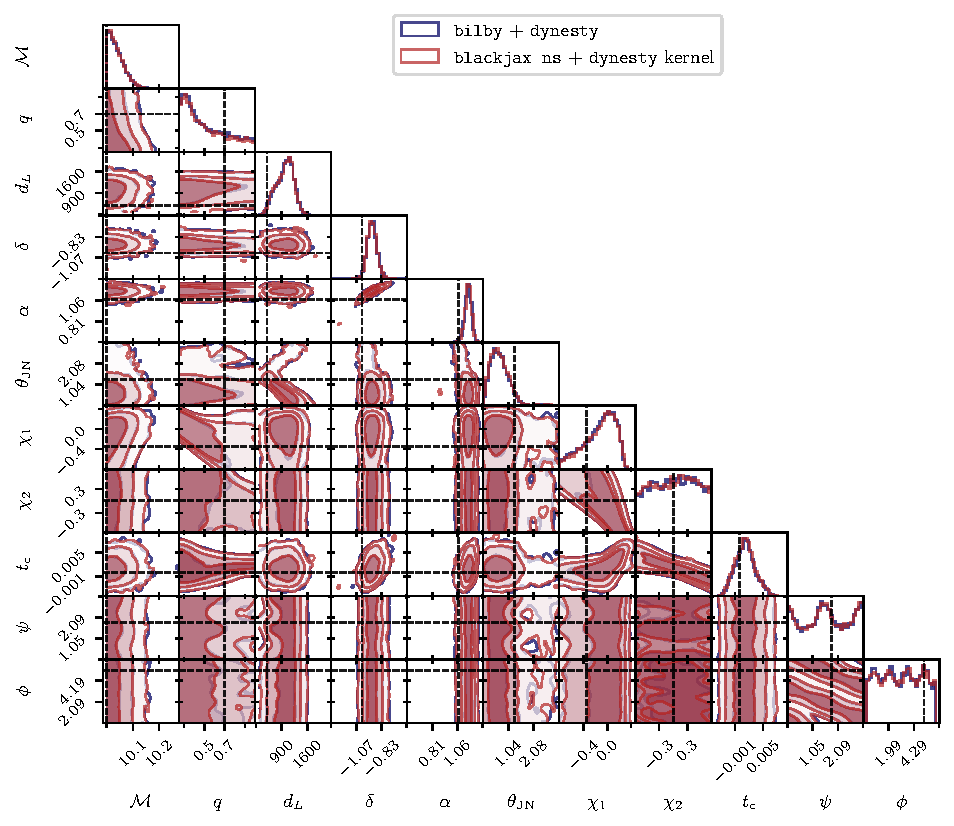
\includegraphics{figures/8s_corner_comparison.pdf}
    \caption{Recovered posterior distributions for the 8s simulated
    signal, comparing our GPU-based \texttt{blackjax-ns} sampler
    with the CPU-based \texttt{bilby} sampler. The injected values
    are marked by black lines. The strong statistical agreement confirms
    the validity of our implementation for longer-duration signals.
    Despite requiring more likelihood evaluations for this analysis, the
    GPU implementation still provided a wall-time speedup of
    26.2$\times$ and a cost reduction of 1.64$\times$.}
    \label{fig:8s_posteriors}
\end{figure*}

\begin{figure}
    \centering
    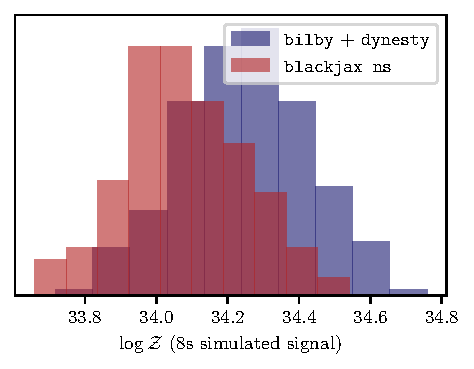
\includegraphics{figures/8s_logZ_comparison.pdf}
    \caption{Comparison of the recovered log-evidence ($Z$) for the 8s
    signal. The results from both the \texttt{bilby} and
    \texttt{blackjax-ns} frameworks are consistent within their
    estimated numerical uncertainties.}
    \label{fig:8s_logZ}
\end{figure}

The recovered posterior distributions and log-evidence values are shown
in Figure~\ref{fig:8s_posteriors} and Figure~\ref{fig:8s_logZ}. We again
find excellent agreement between the two frameworks, further validating
the accuracy of our implementation, despite the differences arising from 
parallelisation. The CPU-based \texttt{bilby} analysis required 167.2 total CPU-hours to
converge, performing 58 million likelihood evaluations. Our GPU-based
\texttt{blackjax-ns} sampler completed the same analysis in 6.37 hours,
corresponding to a wall-time speedup factor of $\times$26.2. This was
achieved despite performing 140 million likelihood evaluations, more than
double that of the CPU run. This increase is attributable to longer average
MCMC chain lengths in the GPU sampler, a consequence of the
batch-adaptive tuning strategy. In hindsight, we could have reduced the
\texttt{naccept} parameter from 120 to 60 to match the \texttt{bilby} run better for
this signal.
The associated cost-reduction factor for this
analysis was $\times$1.64.

The scaling of the runtime for this longer-duration signal provides a
key insight into the practical limits of GPU parallelisation. In an
ideal model where the GPU has sufficient parallel cores for every
frequency bin, the likelihood evaluation time would be independent of
signal duration. In such a scenario, the total runtime would be dictated
primarily by the number of likelihood evaluations needed for convergence.
In this case, the analysis should only have taken roughly double the time
of the 4-second signal analysis, or $0.8 \times 2 = 1.6$ hours. 
However, we observe that the runtime increased significantly more than
what would be predicted by the increase in likelihood evaluations alone.


This discrepancy arises because the computational load of the larger
frequency array exceeds the parallel processing capacity of the L4 GPU.
As a result, the GPU's internal scheduler must batch the calculation
across the frequency domain, re-introducing a partial serial dependency
that makes the likelihood evaluation time scale with the number of bins.
This result serves as an important practical clarification to a common
argument for GPU acceleration. While the idealised model of
parallelisation suggests that evaluation time should be independent of
signal duration, our work demonstrates that this does not hold
indefinitely. Once the problem size saturates the GPU's finite
resources, such as its compute or memory bandwidth, the runtime once
again begins to scale with the number of frequency bins, a behaviour
analogous to the scaling seen in the CPU-based case.


\section{Conclusions}
\label{sec:conclusions}

In this work, we have presented the development and validation of a
GPU-accelerated implementation of the `acceptance-walk' nested sampling
kernel, a widely used and trusted algorithm within the gravitational-wave
community's standard \texttt{bilby} and \texttt{dynesty} framework. This
particular kernel was chosen as its structure can be adapted to use a
uniform MCMC walk length across all parallel processes in a batch, a
critical feature for avoiding thread divergence and ensuring efficient
execution on GPU hardware. Our implementation leverages the vectorized
nested sampling architecture of \texttt{blackjax-ns} to provide a tool
for rapid, unified Bayesian parameter estimation and model selection.

Through systematic studies of simulated binary black hole signals, we have demonstrated
that our implementation is functionally analogous to the trusted
CPU-based framework, producing statistically consistent posterior
distributions and evidence estimates. The architectural shift to the
GPU yields substantial performance gains, with typical wall-time
speedups of $\times$60-100 and cost reductions of
$\times$4-5 for the problems studied here.

However, the contributions of this work extend beyond the immediate performance
gains demonstrated in our analyses. By developing and validating a
GPU-native implementation of the trusted \texttt{bilby} `acceptance-walk'
kernel, we address two fundamental points regarding the future of
gravitational-wave inference.

First, this work represents a necessary step in future-proofing the
community's core analysis tools. The trajectory of high-performance
computing is increasingly skewed towards GPU-centric architectures, a
trend significantly accelerated by the proliferation of artificial
intelligence and machine learning. The migration of its foundational algorithms to these parallel
architectures is therefore a necessary evolution to ensure they remain
computationally viable with increasing data volumes. Our work provides a direct
and robust pathway for this transition, ensuring that a trusted,
well-understood algorithm remains viable on next-generation hardware.

Second, this work establishes an important
performance baseline. As the community develops novel, GPU-accelerated
sampling algorithms, it is essential to disentangle performance gains
originating from the hardware parallelization itself from those arising
from genuine algorithmic innovation. By developing a functionally
equivalent, GPU-native version of one of the community-standard 
algorithms, we have isolated and quantified the speedup attributable
solely to the architectural shift, which allows for batched sampling and
parallelized likelihood evaluations on a GPU.

This provides a robust reference against which future, more advanced
GPU-based samplers can be rigorously benchmarked. New kernels can now be 
assessed on their own algorithmic merit, beyond
the inherent speedup of the GPU. This work enables a true,
like-for-like comparison between different GPU-based samplers, 
which will be useful for guiding the development
of the next generation of Bayesian inference tools.

There are several future avenues of research and development. 
Having established this performance baseline, we can now rigorously
evaluate novel inner sampling kernels designed specifically for the GPU
architecture. While the fixed MCMC walk length of the `acceptance-walk'
kernel is advantageous for parallelisation, our results highlight a key
challenge: its adaptive tuning strategy, designed for serial execution,
translates sub-optimally to the batched GPU paradigm. This necessitates
manual adjustment of the sampler settings for different problems \DIFaddbegin \DIFadd{and
requires on average longer walks to be performed than in the CPU counterpart}\DIFaddend ,
as the kernel is not natively optimised for this
architecture. This motivates the exploration of alternative inner
sampling kernels, such as those based on the Hit-and-Run Slice Sampling
(HRSS) algorithm introduced in~\cite{yallup2025nested}, which \DIFdelbegin \DIFdel{are
better suited to GPUs and }\DIFdelend may offer
more robust and efficient performance without \DIFdelbegin \DIFdel{problem-specific tuning }\DIFdelend \DIFaddbegin \DIFadd{the same tuning problems}\DIFaddend .

GPU-accelerated sampling algorithms such as the one presented in this work can only run when
paired with a GPU-native likelihood. Our work therefore provides additional motivation for the continued development
and porting of more complex and physically comprehensive waveform models
to GPU-based libraries like \texttt{ripple}. On the software side, future
work will involve integrating additional features from \texttt{bilby}
into our framework, such as the astrophysically motivated prior
distributions for masses, spins, and luminosity distance, to enable 
more realistic analyses that are of interest to the GW community.

Finally, the batched architecture of our sampler is highly compatible
with machine learning techniques used for accelerating Bayesian
inference. Methods that use normalizing flows to speed up
the nested sampling algorithm, such as those in~\cite{Williams2021Nessai} and~\cite{Prathaban}, are most
computationally efficient when they can evaluate a large number of
samples in parallel. The serial nature of a conventional CPU-based
sampler represents a significant bottleneck for these models. In
contrast, our parallel framework is a natural fit for the operational 
requirements of these models. This compatibility enables the development of highly efficient,
hybrid inference pipelines that combine GPU-accelerated sampling with
GPU-native machine learning models, further lowering the computational
cost of future gravitational-wave analyses.

\section*{Acknowledgements}

\DIFdelbegin \DIFdel{The authors would like to thank Ming Yang and Will Templeton for their
invaluable help in the development and testing of early iterations of 
the code applying }\texttt{\DIFdel{blackjax-ns}} %DIFAUXCMD
\DIFdel{to gravitational-wave inference.
}\DIFdelend MP was supported by the Harding Distinguished Postgraduate Scholars Programme (HDPSP). 
This work was partly performed using the Cambridge Service for Data Driven Discovery (CSD3), 
part of which is operated by the University of Cambridge Research Computing on behalf of the
STFC DiRAC HPC Facility (www.dirac.ac.uk). The DiRAC component of CSD3 was funded by BEIS 
capital funding via STFC capital grants ST/P002307/1 and ST/R002452/1 and STFC operations 
grant ST/R00689X/1. DiRAC is part of the National e-Infrastructure.

%%%%%%%%%%%%%%%%%%%%%%%%%%%%%%%%%%%%%%%%%%%%%%%%%%
\section*{Data Availability}

 
\DIFdelbegin \DIFdel{\textcolor{red}{TODO: Add data availability statement.}
}\DIFdelend \DIFaddbegin \DIFadd{All the data used in this analysis, including the relevant nested sampling dataframes, 
can be obtained from~\mbox{%DIFAUXCMD
\cite{Prathaban_2025_zenodo}}\hskip0pt%DIFAUXCMD
. We include a file with all the 
code to reproduce the plots in this paper. The }\texttt{\DIFadd{blackjax-ns}} \DIFadd{code is available 
from~\mbox{%DIFAUXCMD
\cite{blackjax_ns_github}}\hskip0pt%DIFAUXCMD
, and the custom kernel implementated in this paper can
be found at~\mbox{%DIFAUXCMD
\cite{Prathaban_2025_github}}\hskip0pt%DIFAUXCMD
. The latter link also contains instructions and
example files on how to use the kernel to run GW analyses.
}\DIFaddend 



%%%%%%%%%%%%%%%%%%%% REFERENCES %%%%%%%%%%%%%%%%%%

% The best way to enter references is to use BibTeX:

\bibliographystyle{mnras}
\bibliography{references} % if your bibtex file is called example.bib


% Alternatively you could enter them by hand, like this:
% This method is tedious and prone to error if you have lots of references
%\begin{thebibliography}{99}
%\bibitem[\protect\citeauthoryear{Author}{2012}]{Author2012}
%Author A.~N., 2013, Journal of Improbable Astronomy, 1, 1
%\bibitem[\protect\citeauthoryear{Others}{2013}]{Others2013}
%Others S., 2012, Journal of Interesting Stuff, 17, 198
%\end{thebibliography}

%%%%%%%%%%%%%%%%%%%%%%%%%%%%%%%%%%%%%%%%%%%%%%%%%%

%%%%%%%%%%%%%%%%% APPENDICES %%%%%%%%%%%%%%%%%%%%%

\appendix


\section{PP coverage plot for \texttt{bilby} and \texttt{dynesty}}
\label{app:bilby_pp_plot}

For completeness, we present the PP coverage plot for the CPU-based
\texttt{bilby}+\texttt{dynesty} analysis in
Figure~\ref{fig:pp_coverage_bilby}. This serves as a reference for the
corresponding plot for our \texttt{blackjax-ns} implementation shown in
the main text.

As expected for two functionally equivalent samplers, the resulting PP
plot and p-values demonstrate results consistent with
those from our GPU-based framework. We note, however, that while
the two samplers are algorithmically analogous, apart from differences
in the parallelisation strategy, they will not produce
identical results due to their stochastic nature and the inherent
uncertainties in posterior reconstruction from nested sampling.

The primary sources of this variance include the statistical
uncertainty in the weights assigned to the dead points, which are
themselves estimates~\citep{skilling, Higson_Errors}, and an additional
uncertainty inherent to parameter estimation with nested sampling that
is not captured by standard error propagation
methods~\citep{Prathaban_PE_errors}. Consequently, the PP curves and
their associated p-values are themselves subject to statistical
fluctuations. The results from the two frameworks are therefore only
expected to be consistent within these intrinsic uncertainties.
We do not explicitly account for these uncertainties
here, instead leaving this analysis for future work.

\begin{figure}
    \centering
    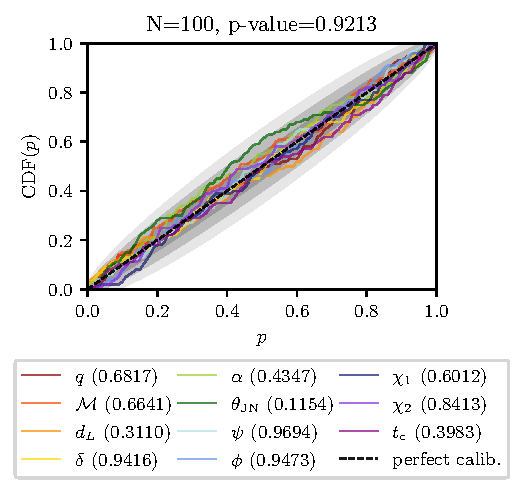
\includegraphics[width=\columnwidth]{figures/pp_coverage_bilby.pdf}
    \caption{PP coverage plot for the 100-injection study, obtained
    with the CPU-based \texttt{bilby+dynesty} sampler. This plot is
    provided for direct comparison with the results from our
    \texttt{blackjax-ns} implementation shown in
    Figure~\ref{fig:pp_coverage}. The results confirm that the CPU-based
    and GPU-based implementations are functionally similar.}
    \label{fig:pp_coverage_bilby}
\end{figure}

\section{Full run statistics for injection study}
\label{app:injection_study_stats}

We present a detailed comparison of the internal sampling statistics for
the 100-injection study in Figure~\ref{fig:injection_study_stats}.
\DIFdelbegin \DIFdel{While the performance metrics such as acceptance rate of the walks are broadly
consistent between the two frameworks}\DIFdelend \DIFaddbegin \DIFadd{Although both sets of runs exhibit similar levels of sample decorrelation
(mean accepted steps per iteration)}\DIFaddend , we observe \DIFdelbegin \DIFdel{instances where }\DIFdelend \DIFaddbegin \DIFadd{that }\DIFaddend the \texttt{blackjax-ns} sampler
\DIFdelbegin \DIFdel{produces significantly longer MCMC chains
paired with lower acceptance rates}\DIFdelend \DIFaddbegin \DIFadd{has a much lower acceptance rate and significantly longer chain lengths}\DIFaddend .    

This behaviour is a direct consequence of the \DIFdelbegin \DIFdel{batch-adaptive tuning
}\DIFdelend \DIFaddbegin \DIFadd{batch sampling
}\DIFaddend strategy, which is fundamental to the GPU implementation. As the nested
sampling run progresses, the live points \DIFdelbegin \DIFdel{can }\DIFdelend \DIFaddbegin \DIFadd{will }\DIFaddend transition into regions of
the parameter space with a very different local likelihood geometry, such that there
is \DIFdelbegin \DIFdel{a sudden shift }\DIFdelend \DIFaddbegin \DIFadd{an increase }\DIFaddend in the difficulty of making moves that are accepted. 
The sequential CPU-based
sampler can adapt to this change immediately by adjusting the walk
length for the very next point. In contrast, the batch-based GPU
sampler only tunes its walk length at the end of a full batch cycle.
\DIFdelbegin %DIFDELCMD < 

%DIFDELCMD < %%%
\DIFdel{If the sampler enters a challenging region shortly after a tuning step,
it must continue with a now-suboptimal (too short) walk length for many
iterations. This results in a sharp drop in the acceptance rate for that
batch. When the tuning is eventually performed, the low average
acceptance rate of the preceding batch triggers a significant,
compensatory increase in the walk length for the subsequent batch. This
mechanism explains the observed correlation between runs with very low
acceptance rates and long MCMC chains}\DIFdelend \DIFaddbegin \DIFadd{It also has a harder likelihood constraint to satisfy for most points,
which further exacerbates the problem}\DIFaddend .

This trade-off between adaptive responsiveness and parallel efficiency
is an inherent characteristic of the batch-based design. Users of this 
framework should therefore always verify that the mean number of
accepted steps per iteration remains sufficiently high for
accurate results. For the injection study presented in this work, we
find that in most of the instances where this effect occurred, the compensatory
increase in chain length was sufficient to maintain an adequate number
of accepted steps. The primary impact was therefore on computational
efficiency (total likelihood evaluations and wall time) rather than the
quality of the posteriors.

\begin{figure*}
    \centering
    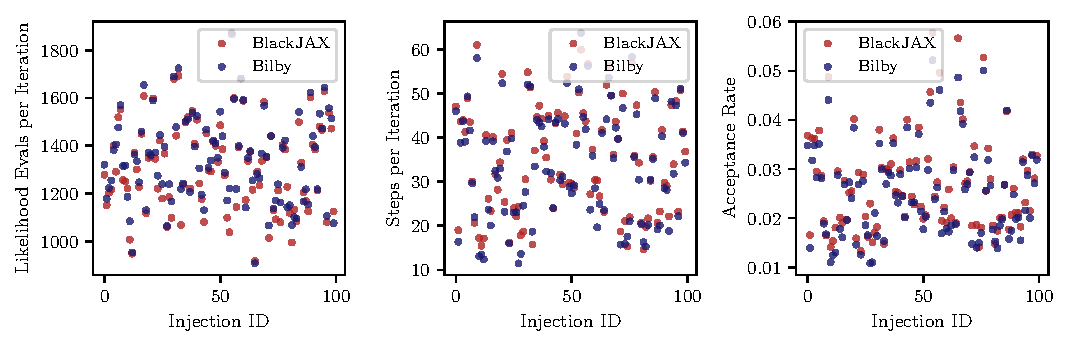
\includegraphics{figures/performance_metrics.pdf}
    \caption{Comparison of internal run statistics for the 100-injection
    study. From left to right: the mean number of MCMC steps (walk length)
    per iteration, the mean number of accepted steps, and the
    mean acceptance rate, for both the \texttt{bilby} and 
    \texttt{blackjax-ns} runs. The batch-adaptive nature of the GPU sampler can \DIFaddbeginFL \DIFaddFL{often
    }\DIFaddendFL lead to \DIFdelbeginFL \DIFdelFL{outlier }\DIFdelendFL runs with longer chains and lower acceptance rates,
    as discussed in Appendix~\ref{app:injection_study_stats}.}
    \label{fig:injection_study_stats}
\end{figure*}

% The full run statistics for the injection study are shown in Figure~\ref{fig:injection_study_stats}.
% In general, the accepted steps per iteration and the acceptance rates
% for both samplers are similar. However, the \texttt{blackjax-ns} sampler
% sometimes exhibits much longer chain lengths and lower acceptance rates,
% skewing the mean accepted steps per iteration lower than the \texttt{bilby}
% runs. This is a consequence of the batch tuning process, where the sampler
% is only tunes every 700 iterations, instead of every iteration as in \texttt{bilby}.
% In both cases, at certain points in the run the samplers will suddenly enter into
% regions of the parameter space that are more difficult to sample, due to
% the complex geometry of the likelihood. In the sequential CPU-based implementation,
% the chain lengths can immediately begin adapt to this shift. However, in the batch-based
% approach, if the live points enter this region soon after a tuning, the chains must wait 
% for potentially hundreds more iterations before the walk lengths can be tuned. This will lead
% to very low acceptance rates for that batch of walks, and then an overcorrection in the 
% walk lengths when the tuning does eventually occur. This is why we sometimes see
% this relationship between very long chain lengths and very low acceptance rates. 
% Unfortunately, since this type of batch tuning is the most natural way to 
% implement the sampler on a GPU, it is difficult to avoid this issue. 
% Users should be aware of this, and make sure that the resulting accepted steps per 
% iteration is not too low regardless, as this will cause the evidences to be inaccurate due
% to overly correlated samples.

% In the case of this injection study, most of the examples where we had much 
% lower acceptance rates than for the \texttt{bilby} runs were cases where the 
% mean chain length was long enough to still result in a similar number of
% accepted steps per iteration, affecting the timing and total likelihood evaluations only,
% not the quality of the results.

% \begin{figure*}
%     \centering
%     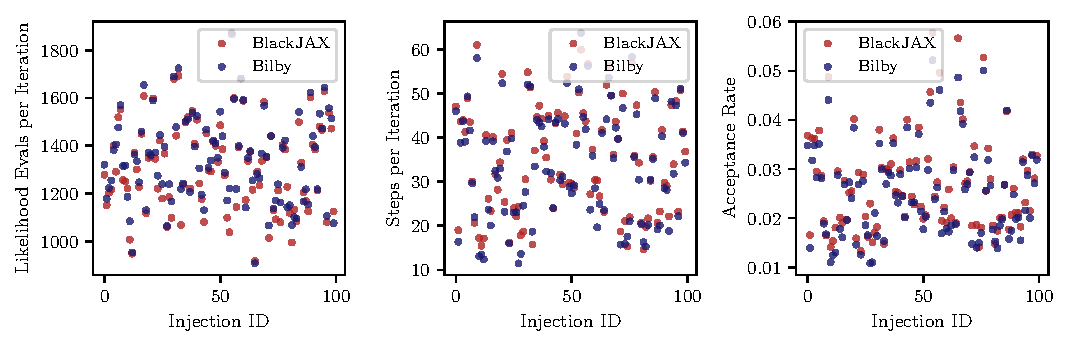
\includegraphics{figures/performance_metrics.pdf}
%     \caption{Full run statistics for the injection study. The
%     \texttt{blackjax-ns} sampler sometimes has much longer chain lengths and 
%     lower acceptance rates than \texttt{bilby} due to the 
%     nature of batch tuning.}
%     \label{fig:injection_study_stats}
% \end{figure*}

%%%%%%%%%%%%%%%%%%%%%%%%%%%%%%%%%%%%%%%%%%%%%%%%%%


% Don't change these lines
\bsp	% typesetting comment
\label{lastpage}
\end{document}